\documentclass[a0paper]{tikzposter}
\usepackage[utf8]{inputenc}
\usepackage{hyperref}
\usepackage{blindtext}

\tikzposterlatexaffectionproofon %shows small comment on how the poster was made



\definecolor{mygray}{HTML}{CCCCCC}
\definecolor{itmGuinda}{RGB}{121,31,37}
\definecolor{itmMoztaza}{RGB}{197, 144, 48}
\definecolor{itmMoztaza2}{RGB}{205, 210, 250}
\definecolor{itmGuinda2}{RGB}{165, 96, 102}
\definecolor{itmGuinda3}{RGB}{214, 180, 183}
% Commands
\newcommand{\bs}{\textbackslash}   % backslash
\newcommand{\itmColor}[1]{{\bf \color{itmGuinda}#1}}   % highlights command

\definecolorstyle{myColorStyle} {
  \definecolor{colorOne}{named}{itmGuinda}
  \definecolor{colorTwo}{named}{itmMoztaza}
  \definecolor{colorThree}{named}{itmGuinda2}
}{
  % Background Colors
  \colorlet{backgroundcolor}{colorTwo!60}
  \colorlet{framecolor}{colorTwo!80}
  % Title Colors
  \colorlet{titlefgcolor}{white}
  \colorlet{titlebgcolor}{colorOne}
  % Block Colors
  \colorlet{blocktitlebgcolor}{colorTwo!50}
  \colorlet{blocktitlefgcolor}{black}
  \colorlet{blockbodybgcolor}{colorTwo!50}
  \colorlet{blockbodyfgcolor}{black}
  % Innerblock Colors
  \colorlet{innerblocktitlebgcolor}{white}
  \colorlet{innerblocktitlefgcolor}{black}
  \colorlet{innerblockbodybgcolor}{white}
  \colorlet{innerblockbodyfgcolor}{black}
  % Note colors
  \colorlet{notefgcolor}{black}
  \colorlet{notebgcolor}{white}
  \colorlet{notefrcolor}{white}
}

\usecolorstyle{myColorStyle}
\usebackgroundstyle{Default}
\usetitlestyle{Wave}
\useblockstyle{Minimal}


\usepackage{avant}
\renewcommand*\familydefault{\sfdefault}
\usepackage[T1]{fontenc}


\title{\textbf{Maestría en Ciencias en Ingeniería Electrónica}}
\author{Instituto Tecnológico de Morelia}
\titlegraphic{
	
\includegraphics[width=15in]{sepLogo.png}\quad 
\includegraphics[width=10in]{tecnmW.png}\quad
\includegraphics[width=5in]{logoITM.png}
	}
\institute{División de Estudios de Posgrado e Investigación}

\begin{document}

% Title block with title, author, logo, etc.
\maketitle

\begin{columns}
  \column{0.33}

  \block[titleoffsety=2cm,bodyoffsety=2cm]{Objetivo de la Maestría}{
    \coloredbox{
    Formar profesionistas con especialización en el área de \itmColor{Procesamiento de Señales} y \itmColor{Electrónica de Potencia}, que logren incorporarse a \itmColor{instituciones de investigación y desarrollo tecnológico, industrias de base tecnológica y a la docencia}.

    }
    %\vspace{0.1in}
    \begin{tikzfigure}
    	%
\includegraphics[width=2in]{uC}
    	
\includegraphics[width=2.5in]{pcb}
    	
\includegraphics[width=2.5in]{osci}
    \end{tikzfigure}
  }
  %=-=-=-=
  \block[titleoffsety=2cm,bodyoffsety=2cm]{Becas}{
    \coloredbox[]{
  	Este programa de maestría cuenta con el reconocimiento del Tecnológico Nacional de México \itmColor{TecNM}, la Secretaría de Relaciones Exteriores \itmColor{SRE}, el programa educativo Roberto Rocca, German Academic Exchange Service \itmColor{DAAD} y el Consejo Nacional de Ciencia y Tecnología \itmColor{CONACyT}, a través del Programa Nacional de Posgrados de Calidad \itmColor{PNPC}, lo que permite postular por becas a estudiantes nacionales y extranjeros, las cuales cubren manutención por un periodo de hasta dos años a los alumnos de tiempo completo que cumplan con los requisitos que exige cada organismo.
    }
   %
   \begin{tikzfigure}
   	
\includegraphics[width=2.5in]{movility.png}
    \end{tikzfigure}
  }
  %=-=-=-=
  \block[titleoffsety=2cm,bodyoffsety=2cm, %titlecenter
  ]
  {Líneas Generadoras del Conocimiento}{
    \coloredbox[bgcolor=itmGuinda3]{
      \begin{itemize}
        \item {\LARGE \itmColor{Electrónica de Potencia}}
        \begin{itemize}
          \item {\bfseries Sistemas de Iluminación}
          \item {\bfseries Calidad de la Energía}
          \item {\bfseries Fuentes Alternas de Energía}
        \end{itemize}
        \item {\LARGE \itmColor{Procesamiento de Señales}}
        \begin{itemize}
          \item {\bfseries Aplicaciones de Telemetría y TICs}
          \item {\bfseries Aplicaciones en Instrumentación y Control}
          \item {\bfseries Sistemas Embebidos}
          \item {\bfseries Redes Inteligentes}
        \end{itemize}
      \end{itemize}

    }
    %
    \begin{tikzfigure}
      
\includegraphics[width=2.5in]{renew}
    	
\includegraphics[width=2.5in]{atom}
      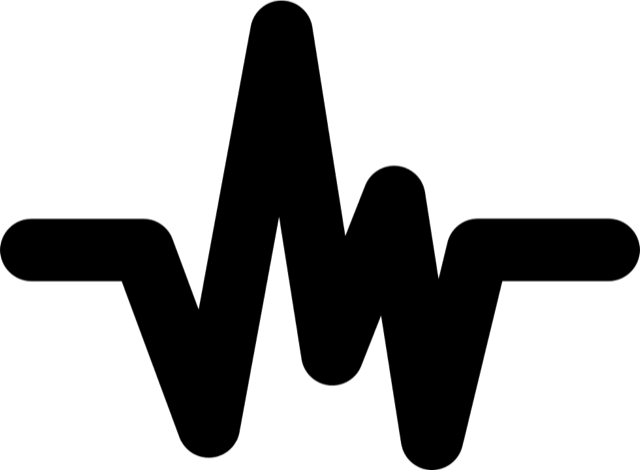
\includegraphics[width=2.5in]{signal}
     \end{tikzfigure}
  }
%*****************************
  \column{0.33}
%=-=-=-=
  \block[titleoffsety=1cm, bodyoffsety=2cm]{Requisitos de Ingreso}{
  \coloredbox{ Para ingresar a la \itmColor{Maestría en Ciencias en Ingeniería Electrónica} se debe:
    \begin{itemize}
      \item Estar titulado de la licenciatura en Ingeniería Electrónica, Ingeniería Eléctrica o área afín con promedio mínimo de 80/100  o equivalente.
      \item Aprobar un exámen de conocimientos en matemáticas y electrónica, o aprobar un curso propedéutico.
      \item Obtener 450 puntos en el examen de inglés del TOEFL.
      \item Aprobar la entrevista personal con docentes de la maestría.
    \end{itemize}
    }
    \begin{tikzfigure}
    	
\includegraphics[width=2.5in]{research}
    	%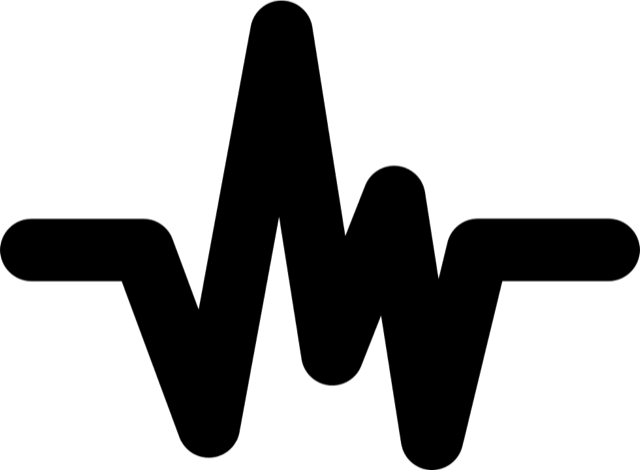
\includegraphics[width=2.5in]{signal}
    \end{tikzfigure}
  }
  %=-=-=-=
  \block[titleoffsety=2cm, bodyoffsety=2cm]{}{
  \coloredbox[bgcolor=itmGuinda3]{
  \begin{itemize}
    \item {\LARGE\itmColor{Documentación Requerida}}
    \begin{itemize}
      \item \bfseries Solicitud de admisión en formato ofical.
      \item \bfseries Título de licenciatura o acta de examen de grado.
      \item \bfseries Copia del certificado de licenciatura.
      \item  \bfseries Copia del acta de nacimiento.
      \item \bfseries Currículum Vitae.
      \item \bfseries Copia de identificación IFE.
      \item \bfseries CURP.
      \item \bfseries Carta de exposición de motivos en formato libre.
      \item \bfseries 2 Cartas de recomendación.
    \end{itemize}
  \end{itemize}
    }
  }
  %=-=-=-=
  %=-=-=-=
  \block[titleoffsety=2cm, bodyoffsety=2cm,titlecenter]{\scshape Información}{
  \coloredbox[bgcolor=itmMoztaza2]{
  \begin{center}
  {\Large\bfseries\centering
  \scshape Instituto Tecológico de Morelia}

    {\centering
      Av. Tecnológico 1500, Col. Lomas de Santiaguito,
      CP 58120, Morelia, Michoacán, México.}

    {\centering
    Tel: (443)312-1570
    }

    %{\centering
    %\scshape División de Estudios de Posgrado e Investigación, Ext. 316
    %}

    {\centering
    \scshape Posgrado en Ingeniería Electrónica,\quad\quad Ext. 330
    }

    {\centering \itmColor{
    \href{mailto:pelectron@itmorelia.edu.mx}{pelectron@itmorelia.edu.mx}}
    }

    {\centering \Large \itmColor{
    \url{www.itmorelia.edu.mx}}
    }

  \end{center}
    }
  }
  %=-=-=-=
  %*****************************
    \column{0.33}
    %=-=-=-=
    \block[titleoffsety=2cm, bodyoffsety=2cm]{Curso Propedéutico}{
    \coloredbox{
        \begin{itemize}
          \item {\itmColor{Requisitos para el Curso}}
          \begin{itemize}
            \item Título de licenciatura o acta de examen de grado.
            \item Solicitud de Admisión.
            \item Pagar costo del proceso de admisión.
          \end{itemize}
          \item {\itmColor{Materias del Curso}}
          \begin{itemize}
            \item Matemáticas
            \item Teoría de Circuitos
            \item Electrónica
            \item Programación Avanzada
          \end{itemize}
        \end{itemize}
        {\bfseries Nota: Las materias se asignan de acuerdo al perfil de ingreso.}
      }
    }
    %=-=-=-=
    %=-=-=-=
    \block[titleoffsety=2cm, bodyoffsety=2cm]{Calendario}{
    \coloredbox{
      \begin{itemize}
        \item \itmColor{Mayo-Agosto}
        \begin{itemize}
          \item \textbf{Mayo:} Inscripción a curso propedéutico y examen$^{*}$.
          \item \textbf{Mayo-Junio:} Curso propedéutico.
          \item \textbf{Junio:} Examen de ingreso y entrevista.
          \item \textbf{Julio:} Publicación de resultados.
          \item \textbf{Agosto:} Inicio de semestre.
        \end{itemize}
        \item \itmColor{Noviembre-Enero}
        \begin{itemize}
          \item \textbf{Noviembre:} Inscripción a curso propedéutico y examen.
          \item \textbf{Noviembre-Diciembre:} Curso propedéutico.
          \item \textbf{Diciembre:} Examen de ingreso y entrevista.
          \item \textbf{Diciembre:} Publicación de resultados.
          \item \textbf{Enero:} Inicio de semestre.
        \end{itemize}
      \end{itemize}
      }
    }
    %=-=-=-=
    %=-=-=-=
    \block[titleoffsety=2cm, bodyoffsety=2cm]{Calendario}{
    \coloredbox{
    %$*:$ Recepción de solicitudes todo el año.

    $*:$ Costo del examen incluido en el pago del proceso de admisión.

    $*:$ Más información en

    \url{http://sagitario.itmorelia.edu.mx/pelectron/Informacion.php}

    }
    \begin{tikzfigure}
      \includegraphics[width=9in]{mcie}
    \end{tikzfigure}
    }
    %=-=-=-=
\end{columns}

\end{document}
